

\section{Project Proposal}
The aim of this project is to design and develop a mathematical model of the most important macroeconomic indicators in the Russian national economy.
The model will be mainly inspired from the macroeconomic model designed and used by the Office of Budget Responsibility (OBR) in the UK \parencite{obr}.
Such model is important for various reasons.
The OBR uses its model for forecasting%
\footnote{\url{https://obr.uk/forecasts-in-depth}}.
They prepare and publish economic forecasts for the purposes of forecasting the public finances \parencite{obr2}.
Examine figure \ref{img:oil-prices} for an example about their forecasting.

\begin{figure}[!htb]
\centering
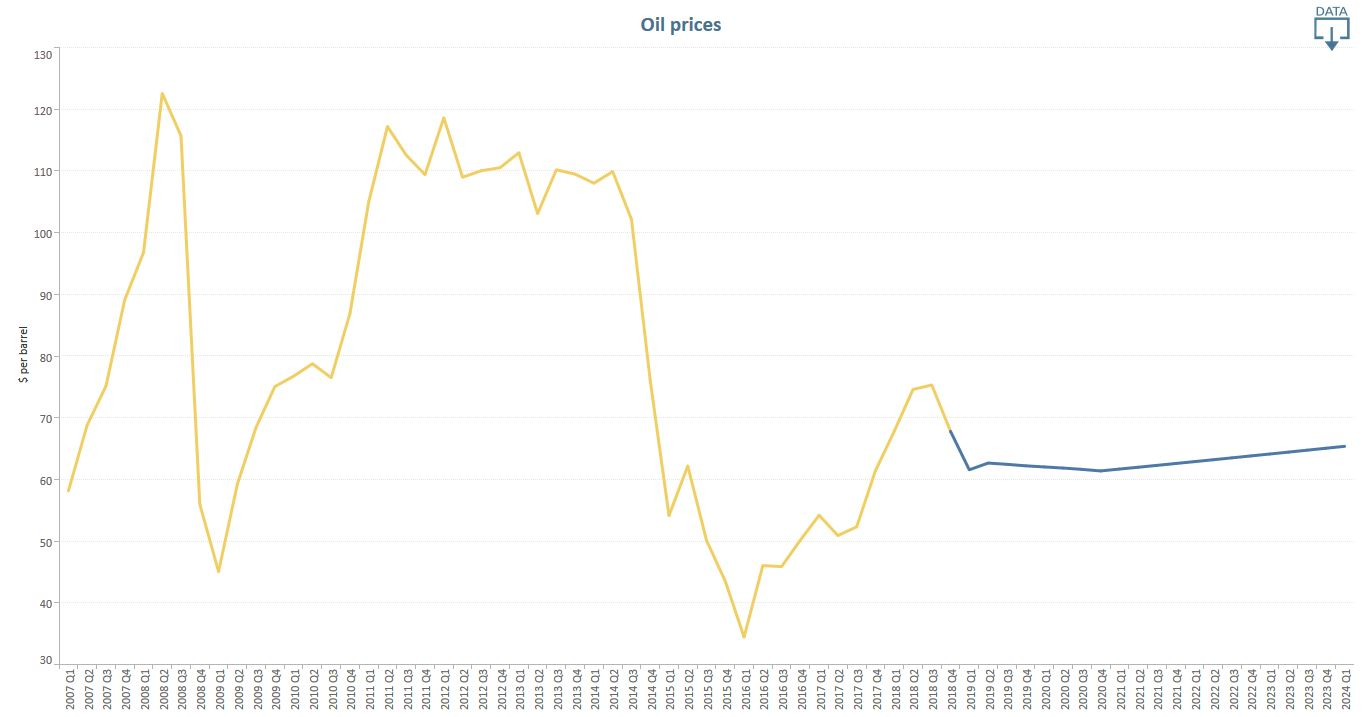
\includegraphics[width=1\textwidth]{images/oil-prices.jpg}
\caption{
UK oil price forecasting by OBR\protect\footnotemark.
The yellow part corresponds to the outturn (real) price recorded,
while the blue part corresponds to the forecasting (predicted) price.
$Q_i$ on the horizontal axis corresponds the $i^{th}$ quarter of the year.
}
\label{img:oil-prices}
\end{figure}

\footnotetext{\url{https://obr.uk/forecasts-in-depth/the-economy-forecast/conditioning-assumptions/\#oilprices}}


